\chapter{Getting started}
\section{Welcome}
This is the manual for Rockbox. Rockbox is an open source firmware replacement
for a growing number of MP3 players. Rockbox aims to be considerably more
functional and efficient than your device's stock firmware while remaining easy
to use and customizable. Rockbox is written by users, for users. Not only is it
free to use, it's also released under the GNU public license, which means that
it will always remain free to both use and to change.

Rockbox has been in development since 2001, and recieves new features, tweaks
and fixes each day to provide you with the best possible experience on your MP3
player. A major goal of Rockbox is to be simple and easy to use, yet remain very
customizable and configurable. We believe that you should never need to go
through a series of menus for an action you perform frequently. We also believe
that you should be able to configure almost anything about Rockbox you could
want, pertaining to functionality. Another top priority of Rockbox is audio
playback quality - Rockbox, for most models, includes a wider range of sound
settings than that device's original firmware. A lot of work has been put into
making Rockbox sound the best it can, and improvements are constantly being made.
All models have access to a large number of plugins, including many games,
applications, and graphical "demos". You can load different configurations
quickly for different purposes (e.g. a large font for in your car, different
sound settings for at home).Rockbox features a very wide range of languages, and
all supported models also have the ability to talk to you - menus can be voiced
and filenames spelled out or spoken.

\section{Getting more help}
This manual is intended to be a comprehensive introduction to the Rockbox
software.
  There is, however, more help available.  The Rockbox website at
\url{http://www.rockbox.org/} contains very extensive documentation and guides
written by members of the Rockbox community and this should be your first port
of call when looking for further help.

\opt{player,recorder,recorderv2fm,ondio}{\section{Before installation}

Before you install Rockbox, you will need to know what model you own.  Rockbox 
comes in different versions depending on the model of your \dap{}.  There are 
six different versions of the software.  The table below will help you to 
identify which version of the software you need.

The model name is printed on the case.  The hard drive size is listed on the
serial number sticker on the back of the unit.

\begin{center}
  \begin{tabularx}{\textwidth}{llXl}\toprule
    \label{ref:Jukeboxtypetable}
    \textbf{Picture} & \textbf{Disk size} & \textbf{Model Name} & \textbf{Version Name} \\\midrule
    \begin{minipage}{2.2cm}
      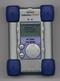
\includegraphics[width=2cm]{getting_started/images/archos-studio-small.png}
    \end{minipage} 
    & 5GB, 6GB, 10GB, 20GB & 
                             \begin{minipage}{8cm}
                             Jukebox 5000 \newline
                             Jukebox 6000 \newline
                             Jukebox Studio 10 \newline
                             Jukebox Studio 20
                             \end{minipage}
                               & player \\\midrule
    \begin{minipage}{2.2cm}
      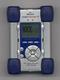
\includegraphics[width=2cm]{getting_started/images/archos-recorder-small.png}
    \end{minipage}
    & 6GB, 10GB, 15GB, 20GB & \begin{minipage}{8cm}
                              Jukebox Recorder 6 \newline
                              Jukebox Recorder 10 \newline
                              Jukebox Recorder 15 \newline
                              Jukebox Recorder 20 
                              \end{minipage}
                               & recorder\\\midrule
    \begin{minipage}{2.2cm}
      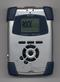
\includegraphics[width=2cm]{getting_started/images/archos-recorderv2-small.png}
    \end{minipage}
                     & 20GB & Jukebox Recorder v2 & recorderv2\\\midrule
    \begin{minipage}{2.2cm}
      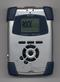
\includegraphics[width=2cm]{getting_started/images/archos-recorderfm-small.png}
    \end{minipage}
                     & 20GB & Jukebox Recorder FM & fmrecorder \\\midrule
    \begin{minipage}{2.2cm}
      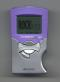
\includegraphics[width=2cm]{getting_started/images/archos-ondiosp-small.png}
    \end{minipage}
                     & 128MB (flash) & Ondio 128 SP & ondiosp \\\midrule
    \begin{minipage}{2.2cm}
      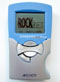
\includegraphics[width=2cm]{getting_started/images/archos-ondiofm-small.png}
    \end{minipage}
                     & 128MB (flash) & Ondio 128 FM & ondiofm \\\bottomrule
  \end{tabularx}
\end{center}
\note{Rockbox does not run on the Archos Jukebox Multimedia or any
Archos products other than those mentioned here.}
}
\opt{h1xx,h300}{% $Id$ %
\subsection{Installing the bootloader}
  Installing the bootloader is the trickiest part of the installation.
  The Rockbox bootloader allows users to boot into either the Rockbox 
  firmware or the iriver firmware. For legal reasons, we cannot distribute 
  the bootloader. Instead, we have developed a program that will patch the 
  Iriver firmware with the Rockbox bootloader. These instructions will explain 
  how to download and patch the Iriver firmware with the Rockbox bootloader 
  and install it on your jukebox.

\begin{enumerate}
  \item Download a supported version of the Iriver firmware for your 
  \playername\ from the Iriver website or from 
  \wikilink{ManualRockboxInstall}.
  Supported Iriver firmware versions currently include 
  \opt{IRIVER_H100_PAD}{1.63US, 1.63EU, 1.63K, 1.65US, 1.65EU, 1.65K, 1.66US, 
    1.66EU and 1.66K.  Note that the H140 uses the same firmware as the H120;
    H120 and H140 owners should use the	firmware called \fname{ihp\_120.hex}.
    Likewise, the iHP110 and iHP115 use the same firmware, called 
    \fname{ihp\_100.hex}.   Be sure to use the correct firmware file for 
    your player.}
  \opt{IRIVER_H300_PAD}{1.28K, 1.28EU, 1.28J, 1.29K, 1.29J and 1.30EU.
    \note{The US H3xx firmware is not currently supported and cannot be
    patched to be used with the bootloader. If you wish to install Rockbox
    on a US \playername\, you must use an international firmware, which will
    permanently remove DRM support from the player.}
  }
  If the file that you downloaded is a \fname{.zip} file, use an unzip 
  utility such as \fname{InfoZip}, \fname{7zip}, \fname{WinRAR},	or 
  \fname{WinZip} to extract the \fname{.hex} from the \fname{.zip} file
  to your desktop. Likewise, if the file that you downloaded is an 
  \fname{.exe} file, double-click on the \fname{.exe}	file to extract 
  the \fname{.hex} file to your desktop.
  %
  \item Download the firmware patcher \fname{fwpatcher.exe} from 
  \url{http://download.rockbox.org/bootloader/iriver/} and save it to your desktop.
    \warn{The firmware patcher contains Unicode support, which is not supported by 
    all versions of Windows. If you have difficulty with the firmware patcher, try 
    downloading the alternate firmware patcher \fname{fwpatchernu.exe}, which is 
    built without Unicode support.}
  %
  \item Go to your desktop and double-click on whichever version of the firmware 
  patcher you downloaded in the prior step.
  %
  \item In the firmware patcher dialog box, click on the BROWSE button and navigate
  to the \fname{.hex} file that you previously downloaded to your desktop.
  %
  \item Click PATCH. The firmware patcher will patch the original firmware to 
  include the Rockbox bootloader. The \fname{.hex} file on your desktop is now
  a modified version of the original \fname{.hex} file.
  %
  \item Turn on your \playername\ and connect it to your computer via USB.
  %
  \item Copy or move the modified \fname{.hex} file to the ROOT directory of 
    your jukebox.
  %
  \item Disconnect the jukebox from USB. (Be sure to use Windows' ``safely remove
  hardware'' option.)
  \warn{Before proceeding further, make sure that your player has a full charge, 
    or that it is connected to the power adaptor.}
  %
  \item Update your \playername s firmware with the patched bootloader. To do this, turn 
    the jukebox on. Press and hold the 
    \opt{IRIVER_H100_PAD}{\ButtonSelect{} button }%
    \opt{IRIVER_H300_PAD}{\ButtonSelect{} button }%
    to enter the main menu, and navigate to \setting{General $\rightarrow$ Firmware 
    Upgrade}. Select \setting{Yes} when asked to confirm if you want to upgrade the 
    firmware. The \playername{} will display a message indicating that the
    firmware update 
    is in progress. Do not interrupt this process. When the firmware update is 
    complete, the player will turn itself off. (The update firmware process usually 
    takes a minute or so.)

    You have now installed the Rockbox bootloader. 

\opt{h1xx}{\note{If you install the Rockbox bootloader, but do not install the
  Rockbox firmware, the Rockbox bootloader will load the iriver firmware when the
  jukebox is turned on.}}

\end{enumerate}
}

\section{Downloading Rockbox}
The latest release of the Rockbox software will always be available from
\url{http://www.rockbox.org/download/}.
\opt{MASCODEC}{
  Windows users may wish to download the self{}-extracting Windows installer,
  which works for all Jukebox models, but those wishing to install manually or
  using a different operating system should choose the .zip archive containing
  the firmware for their model of the Jukebox.
}

\section{Installing Rockbox}\label{sec:installing_rockbox}
\opt{MASCODEC}{
  Using the Windows self installing executable to install Rockbox is the easiest
  method of installing the software on your Jukebox.  Simply follow the
  on{}-screen instructions and select the appropriate drive letter and Jukebox
  model when prompted.  You can use ``Add / Remove Programs'' to uninstall the
  software at a later date.
}
\opt{SWCODEC}{
  \fixme{INCLUDE INSTALL INSTRUCTIONS FOR IRIVERS, IPODS, IAUDIO HERE.}
}
For non{}-Windows users and those wishing to install manually from the archive
the procedure is still fairly simple.  Connect your \playername\ to the
computer via USB as described in the manual that came with your \playername. On
Windows, the \playername\ drive will appear as a drive letter in your
``My Computer'' folder. Take the file that you downloaded above, and unpack
its contents to your \playername\ drive. You can do this using a program such
as \url{http://www.info-zip.org/} or \url{http://www.winzip.org/}.

You will need to unpack all of the files in the archive onto your hard disk. If
 this has been done correctly, you will have a file called 
\fname{\firmwarefilename} in the main folder of your \playername\ drive, and
also a folder called /\fname{.rockbox}, which contains a number of system files
used by the software.

\section{Enabling Speech Support (optional)}\label{sec:enabling_speech_support}
If you wish to use speech support you will also need a language file, available
from \url{http://www.rockbox.org/twiki/bin/view/Main/VoiceFiles/}.  For the
English language, the file is called \fname{english.voice}. When it has been
downloaded, unpack this file and copy it into the \fname{lang} folder which is
inside the /\fname{.rockbox} folder on your Jukebox. Voice menus are turned on
by default. See page \pageref{ref:Voiceconfiguration} for details on voice
settings.


\section{Running Rockbox}
Remove your Jukebox from the computer's USB port. Unplug any connected power
supply and turn the unit off. When you next turn the unit on, the Jukebox
firmware will start to load, and then it will load Rockbox for you. When you see
the Rockbox splash screen, Rockbox is loaded and ready for use.

\section{Uninstalling Rockbox}
If you would like to go back to using the original \playername\ software, then
connect the \playername\ to your computer, and delete the
\fname{\firmwarefilename} file. If you wish to clean up your disk, you may also
wish to delete the \fname{.rockbox} folder and its contents. Turn the
\playername\ off and on and the normal \playername\ software will load.
